\newpage
\section{Auswertung}
\label{sec:Auswertung}

Die gegebenen Werte für \(L\), \(C\) und \(C_{sp}\) sind:
\begin{table}
  \centering
  \caption{Gegebene Werte}
  \label{tab:tab}
  \begin{tabular}{c c}
    \midrule
    \(L\) & \(3.2351\cdot10^{-2} H\)\\
    \(C\) & \(8.015\cdot10^{-10} F\)\\
    \(C_{sp}\) & \(3.7\cdot10^{-11} F\)\\
    \bottomrule
  \end{tabular}
\end{table}

\subsection{Verhältnis von Schwingungs- und Schwebungsfrequenz}
Die Anzahl der Maxima in einer Einhüllenden steigt mit der Kapazität an, wie \autoref{fig:plot} zeigt.
\begin{table}
  \centering
  \caption{Tabelle der Messwerte zur Schwingungsfrequenz}
  \label{tab:tab1}
  \begin{tabular}{c c c}
    \toprule
    \(C_K\) in $nF$ & Anzahl Maxima & Anzahl Minima\\
    \midrule
    2.03 & 4 & 3\\
    3.00 & 5 & 4\\
    4.00 & 5 & 6\\
    5.02 & 6 & 7\\
    6.47 & 8 & 8\\
    8.00 & 11 & 10\\
    9.99 & 14 & 13\\
    \bottomrule
  \end{tabular}
\end{table}

%In \autoref{fig:plot} sieht man, die Messwerte und eine Ausgleichsgerade. 
\begin{figure}
  \centering
  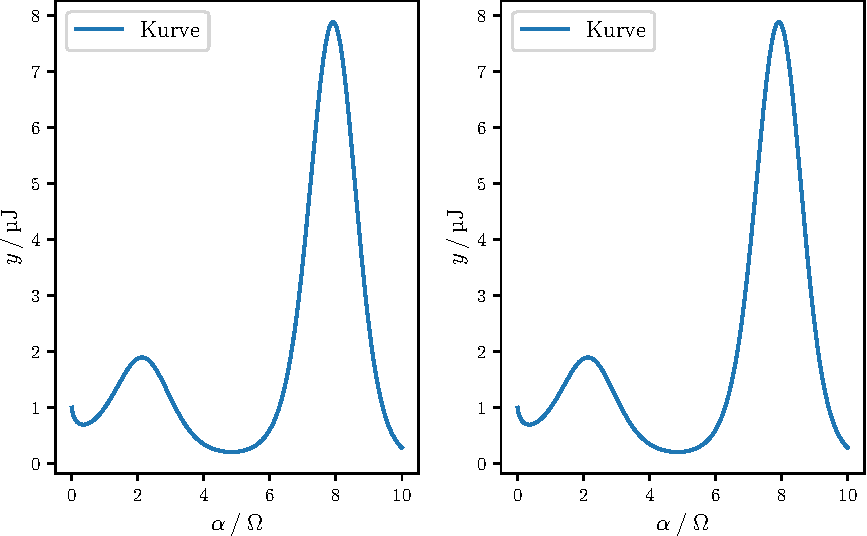
\includegraphics{plot.pdf}
  \caption{Kapazität gegen Anzahl an Extrema.}
  \label{fig:plot}
\end{figure}
\newpage
Das Verhältnis muss demnach annähernd linear mit der Kapazität ansteigen.
Die rechnerischen Werte für \(\nu_+\) ergeben sich aus:
\begin{equation}
  \nu_+ = \frac{1}{\sqrt{LC}} = 196.3832kHz
\end{equation}
\centering{oder}
\begin{equation}
  \nu_+ = \frac{1}{\sqrt{L(C+C_{sp})}} = 192.0015kHz
\end{equation}
Um das theoretische Verhältnis zu ermitteln, werden die Theorie-Werte aus \autoref{tab:tab3} durch die errechnete Schwebungsfrequenz von 192.0015kHz geteilt.

\begin{table}
  \centering
  \caption{Theoretisches Schwingungsverhältnis.}
  \label{tab:tab6}
  \begin{tabular}{c c}
    \toprule
    \(C_K\) in $nF$ & Verhältnis \(\frac{\nu_-}{\nu_+}\)\\
    \midrule
    2.03 & 0.215\\
    3.00 & 0.199\\
    4.00 & 0.19\\
    5.02 & 0.184\\
    6.47 & 0.179\\
    8.00 & 0.175\\
    9.99 & 0.172\\
    \bottomrule
  \end{tabular}
\end{table}

Die Anzahl der Maxima repräsentiert ebenfalls das Verhültnis, indem die Division:
\ \\
\centering{\(\frac{1}{Anzahl Maxima}\)}\\
\ \\
durchgeführt wird.
\\
\newpage
Dafür ergeben sich dann folgende Werte:

\begin{table}
  \centering
  \caption{Experimentelles Schwingungsverhältnis.}
  \label{tab:tab7}
  \begin{tabular}{c c}
    \toprule
    \(C_K\) in $nF$ & Verhältnis mit Maxima\\
    \midrule
    2.03 & 0.25\\
    3.00 & 0.2\\
    4.00 & 0.2\\
    5.02 & 0.166\\
    6.47 & 0.125\\
    8.00 & 0.091\\
    9.99 & 0.71\\
    \bottomrule
  \end{tabular}
\end{table}
Zu Anfang scheinen die Messwerte noch gut übereinzustimmen, aber ab einer Kapazität von 6.47nF betragen die Unterschiede bereits über 30\%.

\newpage
\subsection{Lissajou-Figuren}

\begin{table}
  \centering
  \caption{Tabelle der Messwerte zur Phasenverschiebung}
  \label{tab:tab2}
  \begin{tabular}{c c c}
    \toprule
    \(C_K\) in $nF$ & \(\nu_-\) in $Hz$ & \(\nu_+\) in $Hz$\\
    \midrule
    1.01 & 47090 & 30450\\
    2.03 & 39990 & 30440\\
    3.00 & 37275 & 30440\\
    4.00 & 35730 & 30440\\
    5.02 & 34760 & 30440\\
    6.47 & 33870 & 30440\\
    8.00 & 33260 & 30440\\
    9.99 & 32740 & 30440\\
    \bottomrule
  \end{tabular}
\end{table}

\autoref{fig:plot2} zeigt die Frequenzen, bei denen unter verschiedenen Kapazitäten die Phasenverschiebung 0 beträgt, also \(\nu_-\), oder \(\pi\), also \(\nu_+\).
Es ist sehr deutlich zu sehen, dass die Phasenverschiebung um \(\pi\) so gut wie immer bei der selben Frequenz erfolgt, unabhängig von der Kapazität.
\(\nu_-\) hingegen fällt mit zunehmender Kapazität exponentiell ab.
\begin{figure}
  \centering
  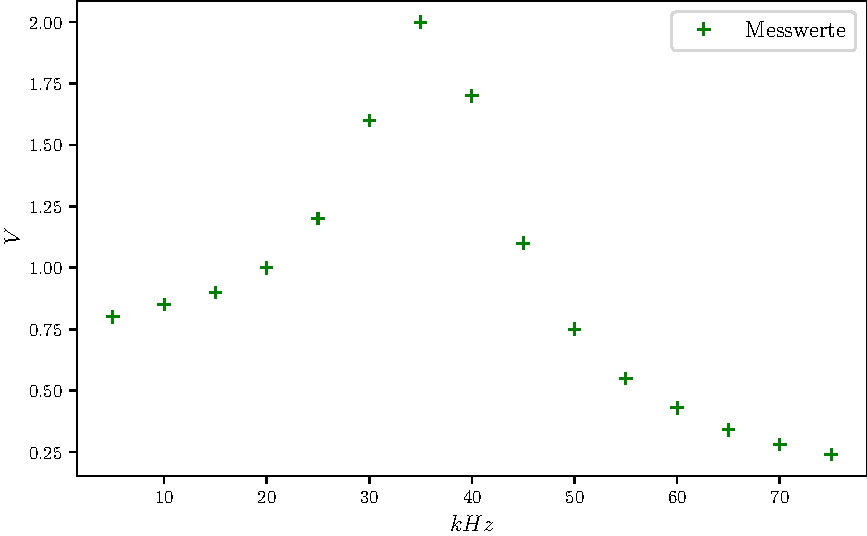
\includegraphics{plot2.pdf}
  \caption{Kapazität gegen Frequenz.}
  \label{fig:plot2}
\end{figure}
\newpage
Die Theorie-Werte für \(\nu_-\) weichen nur leicht ab:
\\
\begin{table}
  \centering
  \caption{Theoriewerte für \(\nu_-\)}
  \label{tab:tab3}
  \begin{tabular}{c c}
    \toprule
    C in \(nF\) & \(\nu_-\) in \(Hz\)\\
    \midrule
    1.01 & 49842.28\\
    2.03 & 41294.10\\
    3.00 & 38154.68\\
    4.00 & 36404.43\\
    5.02 & 35294.99\\
    6.47 & 34290.31\\
    8.00 & 33608.58\\
    9.99 & 33023.39\\
  \end{tabular}
\end{table}
Die Abweichungen von den gemessenen Werten verkleinern sich mit zunehmender Kapazität \(C_k\), angefangen bei 5.52\% bei 1.01nF bis hin zu nur 0.86\% bei 9.99nF.
\newpage
\subsection{Stromverlauf im gekoppeltem Schwingkreis}

\begin{table}
  \centering
  \caption{Tabelle der Messwerte zur Phasenverschiebung}
  \label{tab:tab4}
  \begin{tabular}{c c c c c}
    \toprule
    \(C_K\) in $nF$ & Erste Ampl & Zweite Ampl & a in $ms$ & b in $ms$\\
    \midrule
    2.03 & 1.75 & 1.4 & 17.5 & 29.5\\
    3.00 & 1.75 & 1.5 & 18 & 21.5\\
    4.00 & 1.75 & 1.55 & 18 & 16.5\\
    5.02 & 1.75 & 1.55 & 17.5 & 13.5\\
    6.47 & 1.75 & 1.6 & 17.5 & 10.5\\
    8.00 & 1.8 & 1.6 & 17.5 & 8.5\\
    9.99 & 1.8 & 1.6 & 18 & 6.5\\
    \bottomrule
  \end{tabular}
\end{table}

Die \autoref{fig:plot3} zeigt die Verteilung der Frequenzen \(\omega^\pm\) in Anhängigkeit der Kapazität von \(C_k\).
Wie auch schon bei \autoref{fig:plot2} zeigt \(\omega^-\) eine abfallende Kurve.
Um \(\omega^+\) und \(\omega^-\) zu erhalten, muss man die Werte des Wobbelgenerators miteinander verrechnen:
\begin{equation}
  \omega^+ = \frac{24.99 kHz}{0.16 s}\cdot17.5 s \simeq 2733.28 kHz
\end{equation}
\centering{und}
\begin{equation}
  \omega^- = \frac{24.99 kHz}{0.16 s}\cdot 29.5 s + 2733.28 kHz \simeq 7340.81 kHz
\end{equation}
Diese beiden Werte sind bei einer Kapazität von 2.03 nF gemessen worden.
Die selbe Rechnung wird bei allen Kapazitäten angewandt, die man in \autoref{tab:tab5} sieht.

\begin{table}
  \centering
  \caption{Errechnete Frequenzwerte für \(\omega^+\) und \(\omega^-\).}
  \label{tab:tab5}
  \begin{tabular}{c c c}
    \toprule
    \(C_K\) in $nF$ & \(\omega^+\) in $kHz$ & \(\omega^-\) in $kHz$\\
    \midrule
    2.03 & 2733.28125 & 7340.8125\\
    3.00 & 2811.375 & 6169.40625\\
    4.00 & 2811.375 & 5388.46875\\
    5.02 & 2733.28125 & 4841.8125\\
    6.47 & 2733.28125 & 4373.25\\
    8.00 & 2733.28125 & 4060.875\\
    9.99 & 2811.375 & 3826.59375\\
    \bottomrule
  \end{tabular}
\end{table}

\begin{figure}
  \centering
  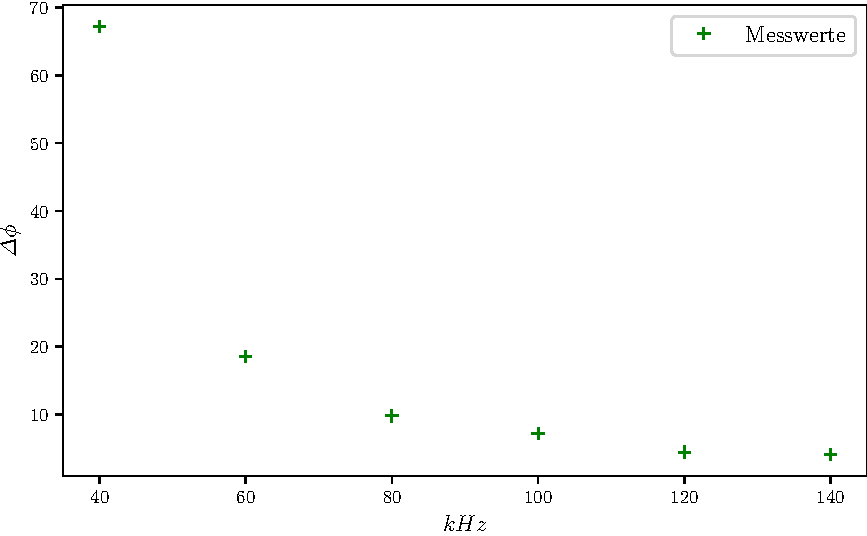
\includegraphics{plot3.pdf}
  \caption{Kapazität gegen Frequenz.}
  \label{fig:plot3}
\end{figure}
Um den zugehörigen Strom zu bestimmen, verwendet man \autoref{eq:strom+} und \autoref{eq:strom-}:
\begin{equation}
  I_2 = |U| \cdot |L(\omega^\pm)| \quad\textrm{mit}\quad |U| = 8V
\end{equation}

\(|L(\omega^\pm)|\) hat bei allen Kapazitäten den ungefähren Wert \(0.01\frac{1}{\Omega}\), sodass \(I_2\) konstant \(0.08A\) ergibt.
